\documentclass{beamer}
\usepackage{beamerthemesplit}
\usepackage{wrapfig}
\usetheme{SPbGU}
\usepackage{pdfpages}
\usepackage{amsmath}
\usepackage{cmap} 
\usepackage[T2A]{fontenc} 
\usepackage[utf8]{inputenc}
\usepackage[english,russian]{babel}
\usepackage{indentfirst}
\usepackage{amsmath}
\usepackage{tikz}
\usepackage{multirow}
\usepackage[noend]{algpseudocode}
\usepackage{algorithm}
\usepackage{algorithmicx}
\usetikzlibrary{shapes,arrows}
\usepackage{fancyvrb}
\usepackage{tikz}
\usepackage{pgfplots}
\beamertemplatenavigationsymbolsempty

\title[]{Комбинирование нейронных сетей и синтаксического анализа для обработки вторичной структуры последовательностей}
\institute[СПбГУ]{
Санкт-Петербургский государственный университет \\
Кафедра системного программирования }

\author[Лунина Полина]{Лунина Полина Сергеевна, 444 группа \\
  \and  
    {\bfseries Научный руководитель:} доцент, к.ф-м.н. Григорьев С.В.
	\and
	{\bfseries Рецензент:} специалист по анализу данных 
	\linebreak ООО "Интеллоджик"  Малыгина Т.С.}

\date{24 мая 2019г.}
\begin{document}
{
% Лого университета или организации, отображается в шапке титульного листа
\begin{frame}
\begin{center}
{
\includegraphics[width=1cm]{pics/logo.jpg}}
\end{center}
\titlepage
\end{frame}
}

\begin{frame}\frametitle{Введение}
\begin{itemize}
    \item Анализ последовательностей, обладающих синтаксической структурой
    \item Существующие подходы:
    \begin{itemize}
        \item N-граммы
        \item Скрытые марковские модели
        \item Ковариационные модели
        \item Вероятностные грамматики
    \end{itemize}
\end{itemize}
\end{frame}

\begin{frame}\frametitle{Постановка задачи}
Цель --- разработка подхода для анализа вторичной структуры последовательностей с использованием комбинации синтаксического анализа и нейронных сетей

\vspace{5\onelineskip}

Задачи:
\begin{itemize}
    \item Разработать архитектуру решения, независимую от конкретной области применения и используемых технологий
    \item Провести экспериментальные исследования
\end{itemize}
\end{frame}

\begin{frame}\frametitle{Описание подхода}
\begin{itemize}
    \item Описание характерных особенностей вторичной структуры исследуемых последовательностей с помощью грамматики
    \item Извлечение этих особенностей с помощью алгоритма синтаксического анализа
    \item Обучение нейронных сетей на полученных данных для решения конкретной задачи
\end{itemize}
\end{frame}

\begin{frame}\frametitle{Генерация данных с помощью синтаксического анализатора}
\begin{itemize}
    \item Входные данные --- грамматика и исследуемые последовательности
    \item Результат работы для входной строки $w$ и нетерминала $N$ --- верхнетреугольная булева матрица разбора $M_N$, где $M_N [i,j] = 1$, если подстрока $w[i,j-1]$ выводима из $N$
    \item Форматы выходных данных:
    \begin{itemize}
        \item Числовые вектора
        \item Черно-белые изображения
    \end{itemize}
\end{itemize}
\end{frame}

\begin{frame}\frametitle{Обучение нейронных сетей}
    \begin{itemize}
        \item Обучение нейронной сети на векторах или изображениях
        \item Для использования обученной модели необходимо снова использовать синтаксический анализатор
        \item Проблема: времязатратность синтаксического анализа
        \item Решение: расширить обученную нейронную сеть верхними слоями, принимающими исходную последовательность
    \end{itemize}
\end{frame}

\begin{frame}{Архитектура решения}
\vspace{6mm}
\hspace*{6mm}
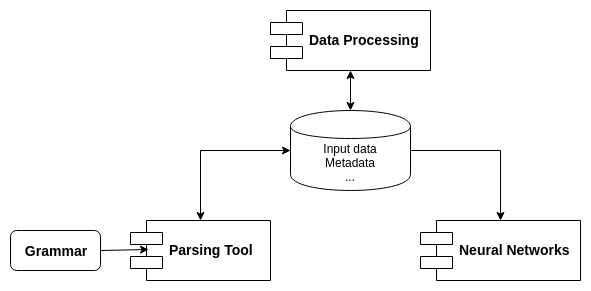
\includegraphics[width=10cm]{pics/arch.png}    
\end{frame}

\begin{frame}\frametitle{Биоинформатика --- область применения}
\begin{itemize}
    \item Задачи анализа нуклеотидных и аминокислотных последовательностей
    \item Шпильки вторичной структуры РНК можно описать грамматикой
\end{itemize} 
\vspace{8mm}
\hspace*{6mm}
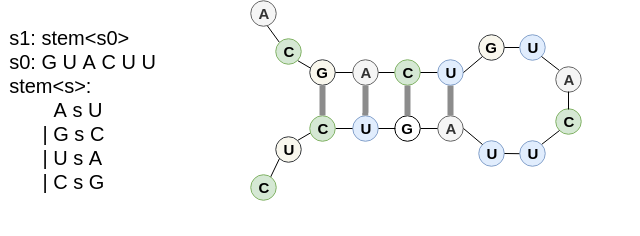
\includegraphics[width=11cm]{pics/rna_gram.png}
\end{frame}

\begin{frame}\frametitle{Эксперименты}
Задачи:
\begin{itemize}
    \item Классификация тРНК эукариотов и прокариотов
    \item Классификация тРНК архей, бактерий, грибов и растений
\end{itemize}
\vspace{6mm}
Технологии:
\begin{itemize}
    \item Платформа YaccConstructor, разработанная на кафедре системного программирования СПбГУ
    \item Библиотека Keras и фреймворк Tensorflow
\end{itemize}
\vspace{6mm}
Базы данных:
\begin{itemize}
    \item tRNADB-CE
    \item Genomic tRNA database
\end{itemize}
\end{frame}

\begin{frame}\frametitle{Эксперименты}
\begin{tabular}{cl}  
    \parbox{0.41\linewidth}{
        \begin{itemize}
            \item Обучение нейронных сетей на векторах и на изображениях
            \item Обучение на их основе нейронных сетей, принимающих исходные последовательности
            \item Тестирование и сравнение результатов
        \end{itemize}
    }
    & \begin{tabular}{l}
            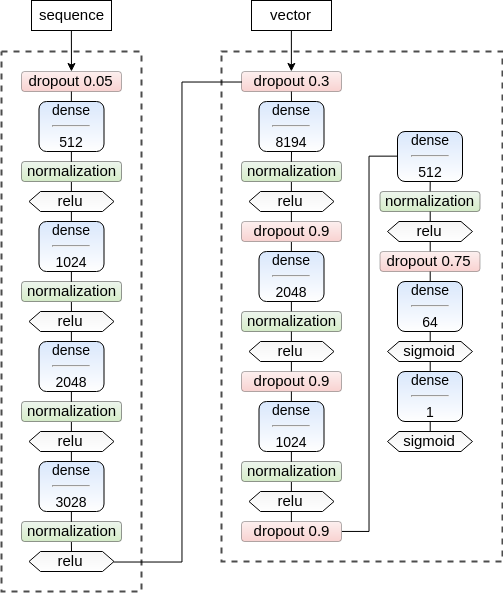
\includegraphics[width=6.5cm]{pics/nn_arch.png}
         \end{tabular}  \\
\end{tabular}
\end{frame}

\begin{frame}\frametitle{Классификация тРНК: эукариоты и прокариоты}
train:valid:test = 20000:5000:10000
\begin{table}[h]
\begin{tabular}{|l|l|l|}
\hline
 accuracy    & vector-based approach & image-based approach \\ \hline
base model   & 94.1\%                & 96.2\%               \\ \hline
extended model & 97.5\%                & 97.8\%               \\ \hline
\end{tabular}
\end{table}
\begin{table}[h]
\begin{tabular}{|l|l|l|l|l|}
\hline
\multirow{2}{*}{class} & \multicolumn{2}{l|}{vector-based approach} & \multicolumn{2}{l|}{image-based approach} \\ \cline{2-5} 
                       & precision             & recall             & precision             & recall            \\ \hline
prokaryotic            & 95.8\%                & 99.4\%             & 96.2\%                & 99.4\%            \\ \hline
eukaryotic             & 99.4\%                & 95.6\%             & 99.4\%                & 99.5\%            \\ \hline
\end{tabular}
\end{table}
\end{frame}

\begin{frame}\frametitle{Классификация тРНК: археи, бактерии, растения и грибы}
train:valid:test = 8000:1000:3000
\begin{table}[h]
\begin{tabular}{|l|l|l|}
\hline
accuracy    & vector-based approach & image-based approach \\ \hline
base model    & 86.7\%                & 93.3\%               \\ \hline
extended model & 96.2\%                 & 95.7\%               \\ \hline
\end{tabular}
\end{table}
\begin{table}[h]
\begin{tabular}{|l|l|l|l|l|}
\hline
\multirow{2}{*}{class} & \multicolumn{2}{l|}{vector-based approach} & \multicolumn{2}{l|}{image-based approach} \\ \cline{2-5} 
                       & precision             & recall             & precision             & recall            \\ \hline
archaeal               & 91.1\%                & 99.2\%             & 91.6\%                & 98.5\%            \\ \hline
bacterial              & 96.6\%                & 95.1\%             & 95.2\%                & 95.5\%            \\ \hline
fungi                  & 98.5\%                & 94.9\%             & 97.5\%                & 94.3\%            \\ \hline
plant                  & 99.4\%                & 95.7\%             & 99.2\%                & 94.7\%            \\ \hline
\end{tabular}
\end{table}
\end{frame}


\begin{frame}\frametitle{Результаты}
\begin{itemize}
    \item Разработана архитектура решения для использования предложенного подхода
    \item Проведены экспериментальные исследования предложенного подхода применительно к следующим задачам биоинформатики:
    \begin{itemize}
        \item Классификация тРНК эукариотов и прокариотов
        \item Классификация тРНК архей, бактерий, грибов и растений
    \end{itemize}
    \item Результаты представлены на конференциях:
    \begin{itemize}
        \item Постер "16s rRNA Detection by Using Neural Networks" на конференции Biata 2018
        \item Статья "The Composition of Dense Neural Networks and Formal Grammars for Secondary Structure Analysis" на конференции BIOINFORMATICS 2019
        \item Постер  "Improved Architecture of Artificial Neural Network for Secondary Structure Analysis" на конференции Biata 2019
    \end{itemize}

\end{itemize}
\end{frame}
\end{document}